\section{Phase 6: Generative Moonshots}

\subsection{Geospatial Fidelity Pivot: From Hexagonal Entropy to Sovereign Containment}

During the validation of the synthetic \texttt{manifold\_v3}, a systemic failure was identified in the distribution of synthetic origins (Pickups). The generative output exhibited high spatial entropy, with synthetic points scattered across regions never historically serviced by the Agent.

\subsubsection{The Resolution Trap: H3 Res 6 vs. Res 9}
Initial attempts to discretize the city used \textbf{Uber H3 Resolution 6} ($\approx 36 \text{ km}^2$). This coarse resolution proved insufficient, conflating high-value strategic sectors with peripheral noise. 

An iterative pivot to \textbf{H3 Resolution 9} (City Block level) was tested to achieve higher precision. However, this introduced a \textit{Sparsity-Overfitting Trap}: the cardinality of unique H3 IDs exceeded the ground-truth volume ($N \approx 4,700$), forcing the GAN to memorize specific coordinates rather than learning the latent "Physics of the Neighborhood."

\begin{figure}[H]
    \centering
    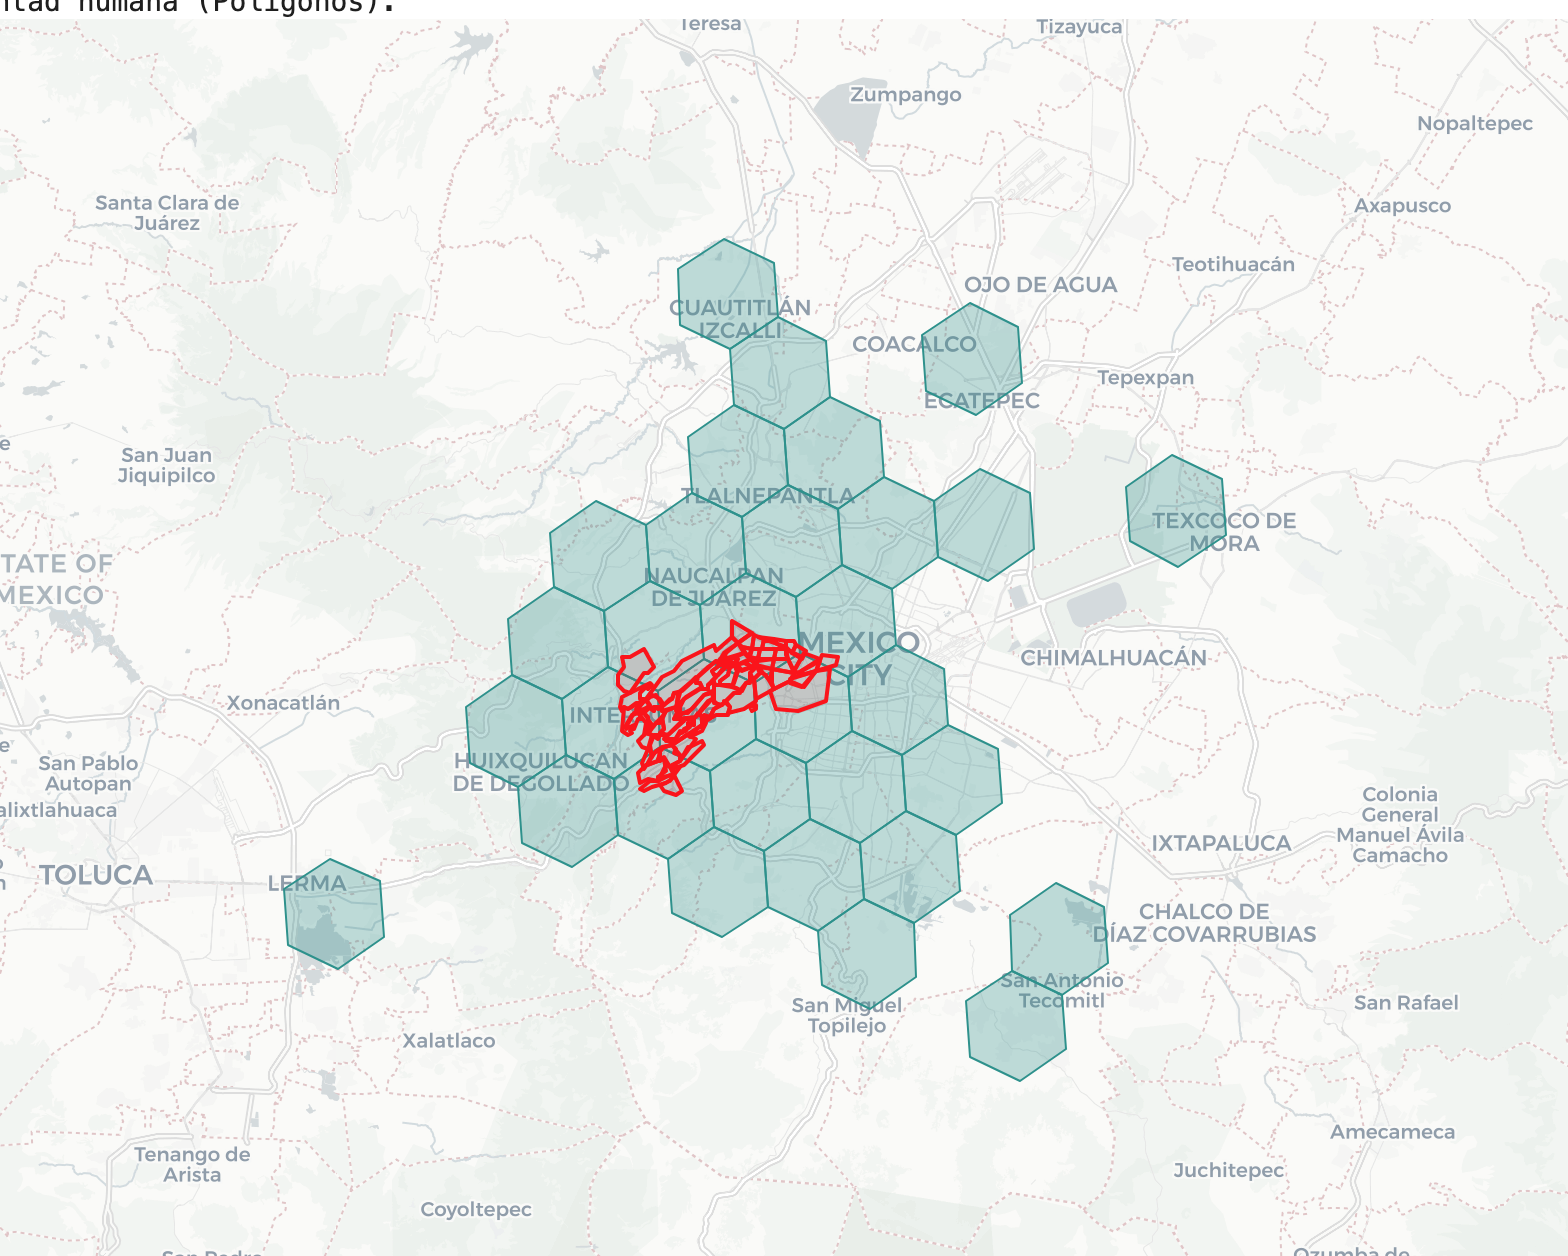
\includegraphics[width=0.8\textwidth]{geo_entropy.png}
    \caption{Visualizing the Resolution Trap: H3 Hexagonal tiling vs. the manually-mapped Sovereign Zone boundaries.}
    \label{fig:geo_entropy}
\end{figure}

\subsubsection{The Sovereign Filter Doctrine}
To resolve the tension between precision and generalization, the purely algorithmic hexagonal approach was deprecated in favor of \textbf{Point-in-Polygon (PiP) Containment}. Field observations confirmed that operational activity is geographically concentrated; any origin outside the manually-mapped 73 polygons (The Sovereign Zone) is statistically an outlier.

\subsubsection{Implementation: The Master Coalesce (v3.0)}
A strict \textbf{Sovereign Axis} filter was implemented for all origin points:
\begin{itemize}
    \item \textbf{Prioritized Mapping:} Pickups within the 73 manual polygons were assigned a semantic ID based on the established hierarchy.
    \item \textbf{Universal Fallback:} All pickups outside these boundaries were relegated to a monolithic \texttt{Unassigned} class.
    \item \textbf{Validation:} A forensic audit confirmed that \textbf{76.7\%} of the real-world operational history resides within the Sovereign Zone, as illustrated in Figure \ref{fig:pickup_heatmap}.
\end{itemize}

\begin{figure}[H]
    \centering
    \begin{subfigure}[b]{0.48\textwidth}
        \centering
        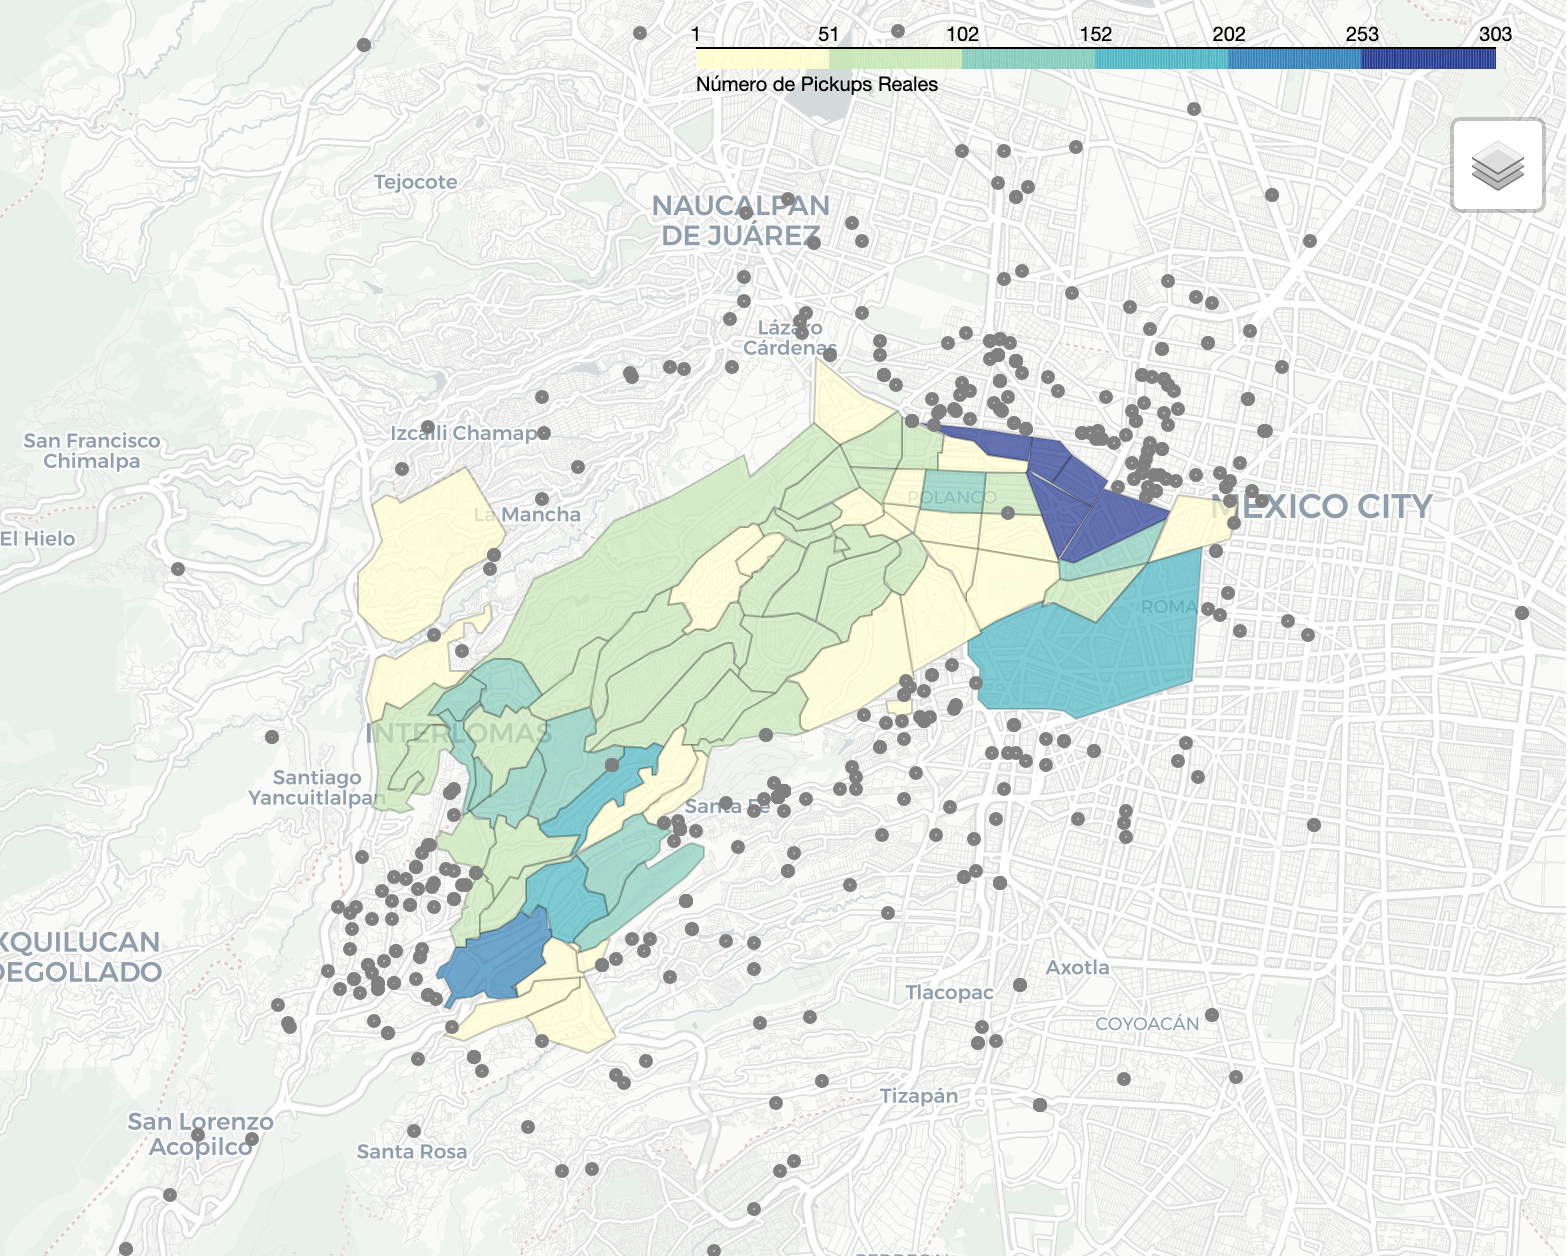
\includegraphics[width=\textwidth]{pickup_heatmap.png}
        \caption{Heatmap of real-world pickups within Sovereign Polygons.}
    \end{subfigure}
    \hfill
    \begin{subfigure}[b]{0.48\textwidth}
        \centering
        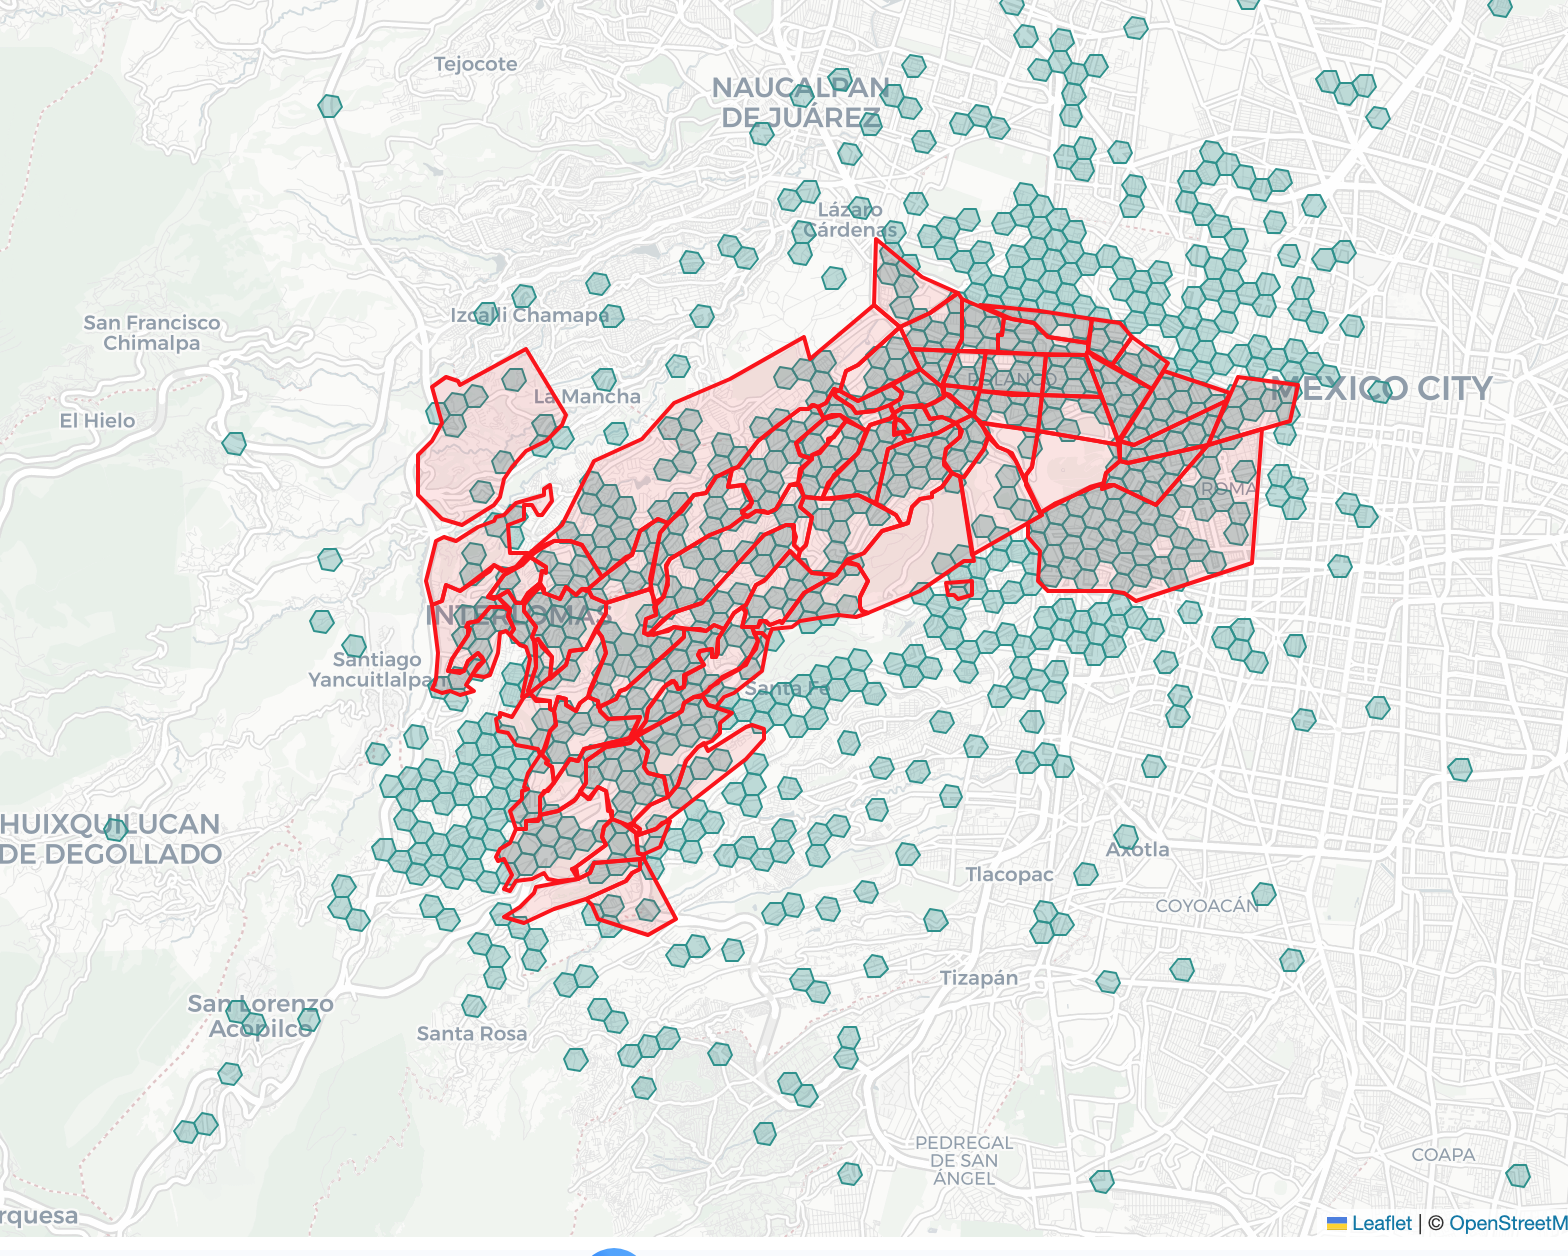
\includegraphics[width=\textwidth]{h3_overlay.png}
        \caption{Refined H3 overlay on the high-signal strategic zone.}
    \end{subfigure}
    \caption{Transitioning from hexagonal entropy to sovereign strategic containment.}
    \label{fig:geospatial_refinement}
\end{figure}

\subsubsection{Significance for GAN v5/v6}
This architectural realignment transforms the Pickup feature from a noisy continuous variable into a \textbf{High-Signal Strategic Indicator}. By distilling the environment into 42 "Islands of Value" and a controlled sea of noise, the GAN is now positioned to learn the precise economic relationships between known origins and known destinations, enabling high-fidelity re-training of the generative manifold.




### 223.3 The Rank-3 Pivot: Temporal Windowing
Unlike XGBoost, the TensorFlow Student will not ingest rows individually. Data will be restructured into **Sliding Windows (Sequences)**.

* **Tensor Shape:** `[BatchSize, LookbackWindow, FeatureVector]`
* **Lookback Window:** $T=5$ (The current offer + the 4 previous offers in the session).
* **The Goal:** By feeding sequences, the model learns to identify "Dry Spells" or "Surge Build-ups," allowing the `reasonprimary` to evolve from a static label to a dynamic state.



### 223.4 The Neural Architecture: The "Memory Bridge"
The proposed architecture (`pienzarnnv1.keras`) will utilize a hybrid structure:

1.  **Input Layer:** Handles the 10-dimensional vector (Fare, Physics, H3/Sovereign IDs).
2.  **LSTM/GRU Layer:** The "Memory Cell." This layer will process the $T=5$ sequence to extract **Market Momentum**.
3.  **Dense Layers (Head):** A series of fully connected layers to perform the final classification (Accept / Reject).
4.  **Softmax Output:** Provides the probability of acceptance.



---

### 223.5 The Transfer Learning Gate (Expert Calibration)
To ensure the model doesn't lose the "Expert Nuance" found only in the real-world data, a two-stage training regime is mandated:

* **Stage 1 (Pre-training):** Train on the 1M Distilled Synthetic rows. The model learns the "General Logic" of the market.
* **Stage 2 (Expert Tuning):** Freeze the early "Physics" layers and fine-tune exclusively on the **4,765 Ground-Truth rows**. This "Expert Calibration" injects the specific, non-synthetic "feel" of Bernardo’s real-world driving into the weights.

### 223.6 Strategic Significance: Toward the "Digital Clone"
This workflow marks the transition from **Predictive Analytics** to **Cognitive Simulation**. By moving to TensorFlow, we are no longer asking *"Will this ride be accepted?"* but rather *"How does the current market flow influence the Agent's strategic threshold?"*

> *// Addendum 223: Architectural Framework Ratified. Transitioning to TensorFlow Submodule 1 for Implementation. //*











# ADDENDUM 225: OPERATION TOPOLOGICAL SOBERANÍA — THE GRAPH NEURAL NETWORK (GNN) PIVOT

**Category:** Advanced Model Architecture & Spatial Connectivity (Phase VII)  
**Status:** `PROPOSED / CONCEPTUAL`  
**Date:** February 17, 2026

---

### 225.1 Context: The Euclidean Limitation
The current **CNN Architecture (Submodule 2/3)** treats Mexico City as a Euclidean grid (pixels/matrices). However, the "Physics of the City" is non-Euclidean. Two points that are physically close in a 2D map (e.g., across a canyon in Santa Fe or a park in Chapultepec) may be topologically distant in terms of transit. 

To capture the **True Connectivity of Profit**, the project proposes a transition from Grid-based to **Graph-based learning**.



---

### 225.2 The Graph Definition: The "Salchichota" Mesh
The city is redefined as a directed graph $G = (V, E)$:

* **Nodes ($V$):** The 73 **Sovereign Polygons**.
    * **Node Features:** Each node carries a 4D vector: `[AvgEPH, SurgeIntensity, DemandDensity, AgentFatigue]`.
* **Edges ($E$):** The road network connectivity.
    * **Edge Weights:** Real-time friction (Time/Distance) between neighboring polygons.
* **Adjacency Matrix ($A$):** A $73 \times 73$ matrix defining the "Sovereign Neighbors."

---

### 225.3 The Mechanism: Message Passing Neural Networks (MPNN)
Unlike the sliding Kernel of a CNN, the GNN uses **Message Passing**.

1.  **Neighborhood Aggregation:** Each polygon (e.g., Anzures) "listens" to the economic state of its neighbors (Polanco, Condesa).
2.  **State Update:** Anzures updates its "Incentive Potential" based on its own state + the economic pressure of the surrounding nodes.



**Result:** The model learns to predict **Latent Opportunity**. It can detect that a zone is about to "explode" in surge before the platform's algorithm even reflects it.

---

### 225.4 Strategic Objective: Spatial Anticipation
The GNN-driven Digital Clone moves from **Reactive Decision** to **Proactive Positioning**:

* **Traditional ML:** "This offer is 100 MXN, I accept."
* **GNN Clone:** "This offer is 100 MXN, but the neighboring node (Polanco) is showing a 20% increase in Message Passing Intensity. I **REJECT** and move 2km North to capture the higher-value surge."

---

### 225.5 Technical Symbiosis: TensorFlow Geometric
The implementation will leverage **TensorFlow GNN** or **Spektral**. This architecture will serve as the "High-Level Strategist" that sits above the sequential LSTM (Addendum 223), creating a multi-layered intelligence system.

---

### 225.6 Significance
This pivot transforms Project Pienza into a **Market Design Simulation**. By modeling the city as a graph, the Architect is no longer just "driving"; he is **navigating the topology of an economic system**. This is the exact technological stack used by Uber's Marketplace team in San Francisco.

> // Addendum 225: Topological Framework Proposed. Concept Ratified for Phase VII. //







FINAL FINAL FINAL

¿Será Posible el Sur? La Negra Sosa's Sur. Bernardo's Utopia.